\chapter{Résultats obtenus par l'application}

\section{Interface graphique}
Vous trouverez ci-joint l'affichage de l'application web avec ces différentes sous parties: "Acceuil" (Figure 6.1), "Commencer"(Figure 6.2 et 6.3), "A Propos" (Figure 6.4).
\subsection{Page d'accueil}
\begin{figure}[H]
  \centering
    
\includegraphics[scale=0.4]{images/resultat_acceuil.jpg}
        \caption{Page d'acceuil}
\end{figure}
\subsection{Page de simulation}
%2 impr : section parametres + section simulation (vide)+ données
\begin{figure}[H]
  \centering
    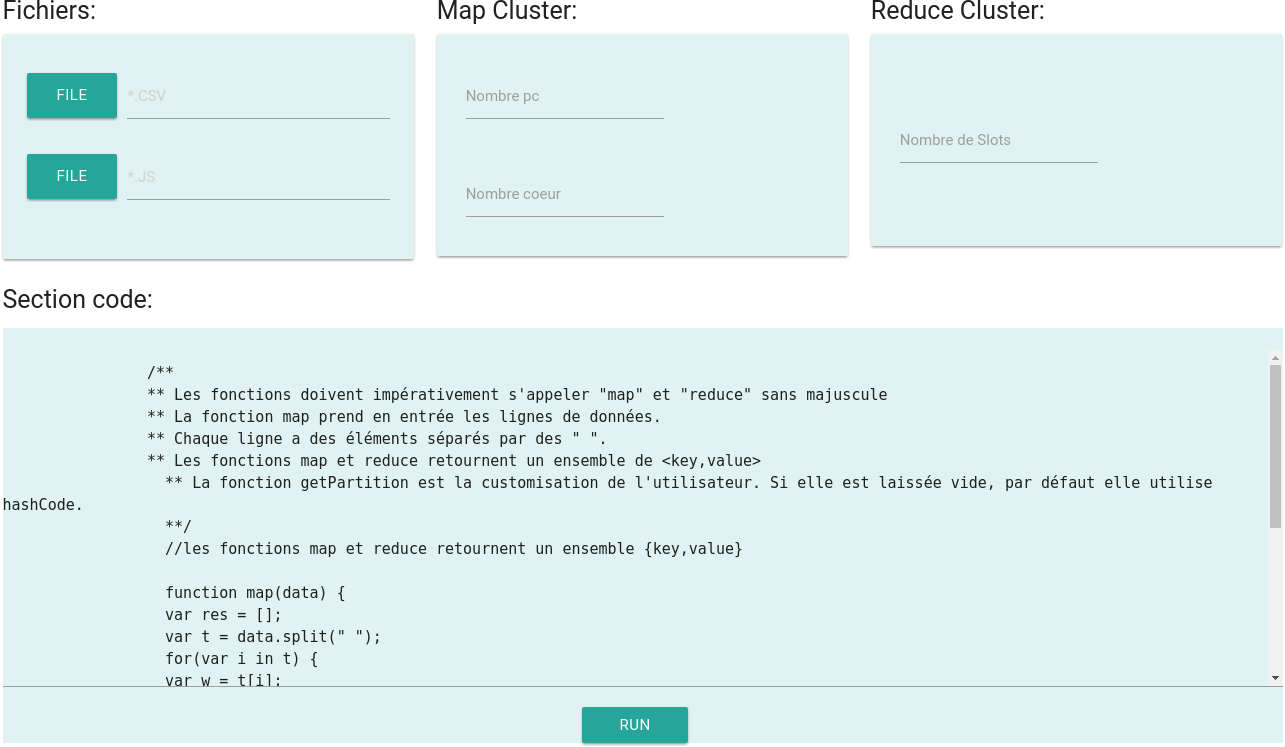
\includegraphics[scale=0.5]{images/resultat_simulation_1.jpg}
        \caption{Simulation - Paramètres}
\end{figure}
\begin{figure}[H]
  \centering
    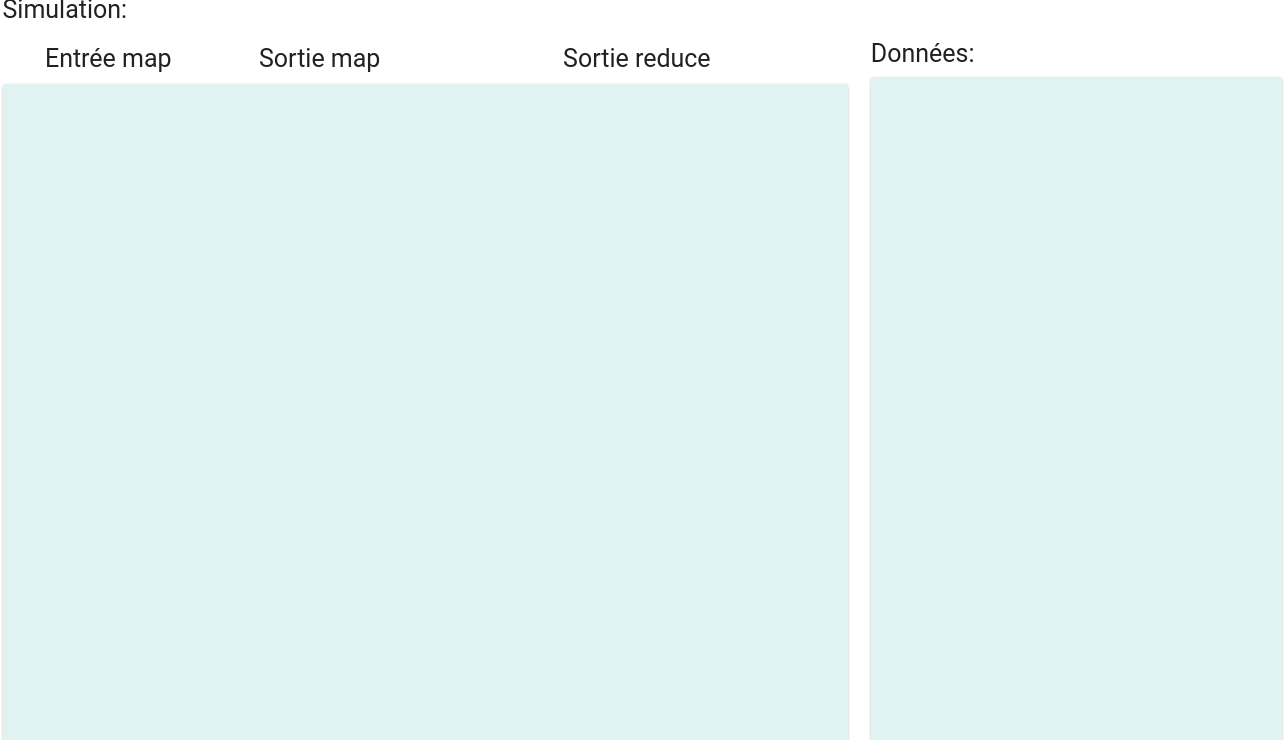
\includegraphics[scale=0.5]{images/resultat_simulation_2.jpg}
        \caption{Simulation - Cluster et données}
\end{figure}

\subsection{Page "A propos"}
\begin{figure}[H]
  \centering
    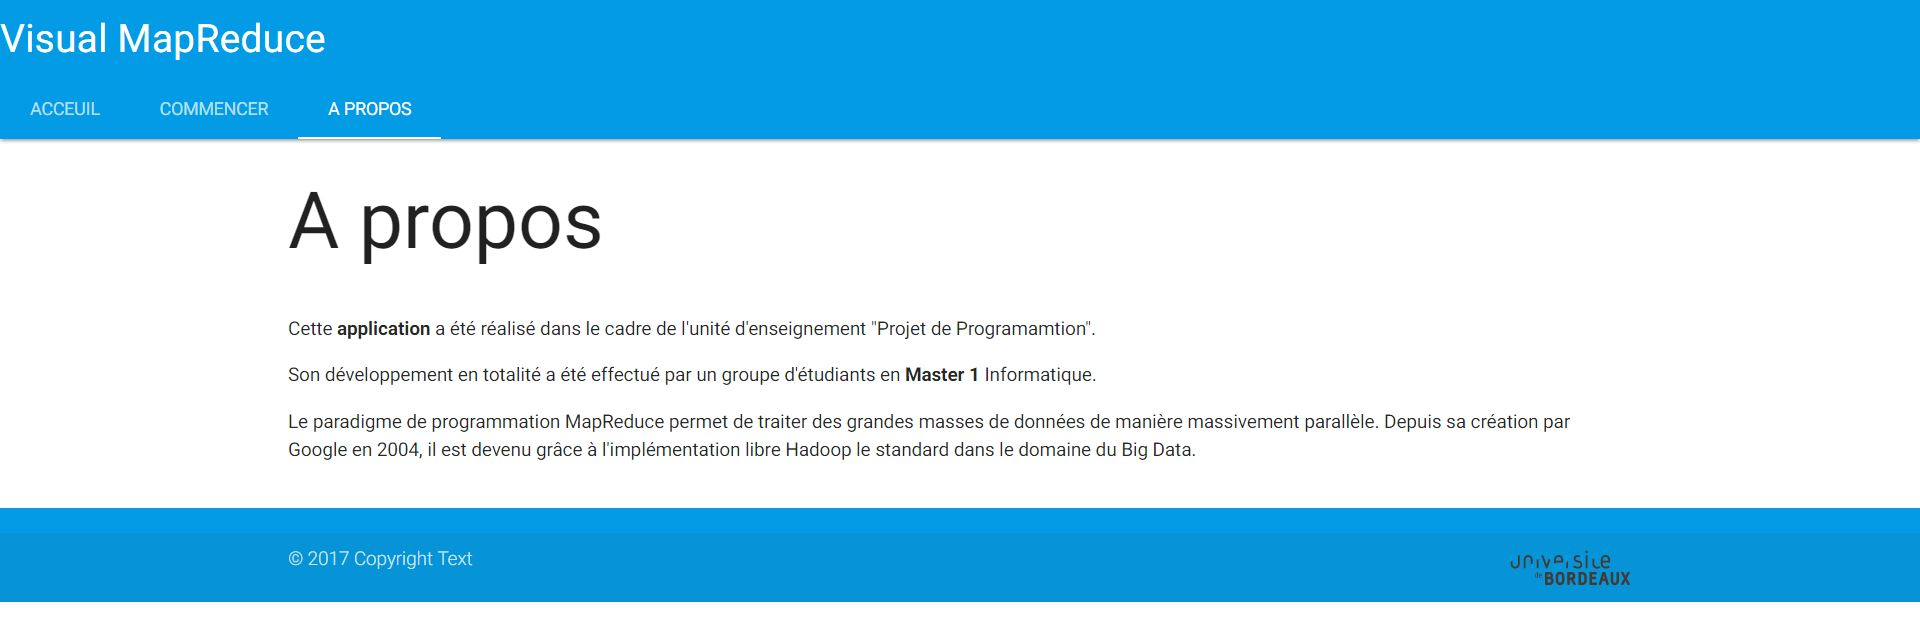
\includegraphics[scale=0.4]{images/apropos.jpg}
        \caption{Page "A propos"}
\end{figure}
\section{Résultats de la simulation}
La simulation (Figure 6.5) est permise grâce à FATuM, ce bloc html est donc uniquement affiché par cette bibliothèque.
\begin{figure}[H]
  \centering
    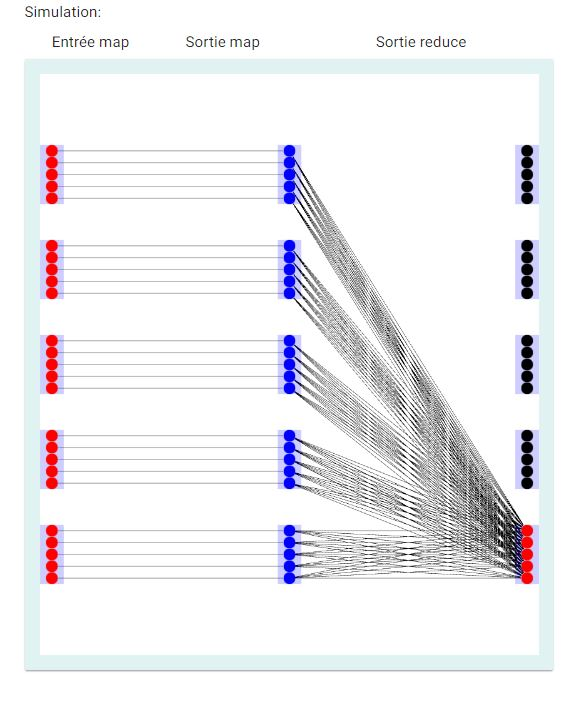
\includegraphics[scale=0.6]{images/resultat_simulation_3.jpg}
        \caption{FATuM}
\end{figure}
\section{Résultats sur console}
Enfin, à la demande du client, nous avons mis les résultats des différentes étapes en sortie de console (Figure 6.3).
\begin{figure}[H]
  \centering
    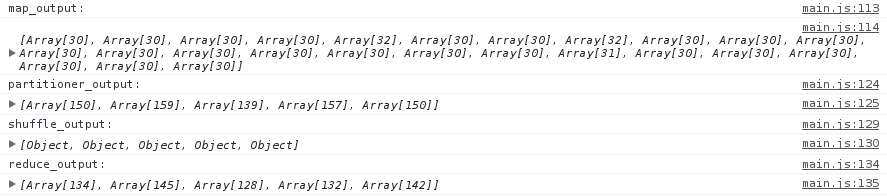
\includegraphics[scale=0.5]{images/resultat_console.png}
        \caption{Sortie Console}
\end{figure}